\acresetall
\chapter{Testbed Implementation}\label{chapter:implementation}\label{ch:implementation}
This chapter depicts the tools and procedures used in the set up and data preparation prior the machine learning procedures. It includes the steps taken since the start of the work until the moment the first \ac{ML} algorithm started to train. First, an overview of the software and hardware tools is given. Afterwards, a short explanation on the available \ac{ML} libraries and frameworks is presented, along with the reasoning behind their choosing for this work. Lastly, process of measuring the data and preprocessing it is explained in detail, for the data to be ready to be applied to the learning models.
\section{Software Defined Radio approach}
As stated in the introduction of this thesis, \ac{SDR} and \ac{CR} play an important role in modern communication systems, and is the framework used for most projects at the \ac{CEL}, not only being used as a tool but also being actively contributed to with research results, but also acting as an active agent on open-source improvements. The software and hardware frameworks used are the following:
\subsection{GNURadio}
\begin{figure}[htb]
    \centering
      
\includegraphics[width=\textwidth]{figures/gnuradio_logo}
      \caption{GNURadio logo}
      \label{fig:gnuradio}
\end{figure}
GNURadio \cite{GNURadio2016} is a free and open-source toolkit that provides a large library of signal processing blocks that can be used for several software-defined radio applications. Its functionality does not require a device in the loop, which allows the users to simulate complete communications systems only on a computer. This includes signal sources, modulators and demodulators (such as \ac{PSK} and even \ac{OFDM}), dynamic channel simulators (and virtually any digital filter implementation), math operators, and a plethora of other digital signal processing implementations that have served purposes in academy, research, amateur radio hobbyist and even some government entities. Additionally, thanks to the support for several defined radio hardware \cite{gnuradiohw}, GNURadio grants the capability of transmitting (given the user has a rightful license for this purpose) and receive real signals and process them thoroughly.\\

The usual usage of this software is as follows: the user has a problem or an idea that requires digital signal processing, such as decoding a radio signal or implementing a novel communications' protocol. As said, GNURadio includes several algorithms that serve this purpose, and they are enclosed in so-called blocks. These blocks can then be connected to one another, generating a flow that the signal follows, in a so-called flowgraph, where each block takes a determinate amount of inputs, each input also taking a determinate amount of samples, that undergo the signal processing that the block entitles, and then the block presents its outputs to the next block downstream. If the library provided by GNURadio does not contain implementations that suffice the user needs, new implementations are easily added by the means of a so-called \emph{\ac{OOT}} module, where the user can provide additional applications, and characteristic that makes the scalability of GNURadio a transparent procedure. Lastly, if the user believes that custom implementation can serve a common purpose and other users, the \ac{OOT} can be made public following the open source standards, and this way other users can benefit from the same implementation and probably even contribute to it. An extensive collection of \ac{OOT} that have followed this open source mentality can be found at \ac{CGRAN} \cite{CGRAN}.\\

Regardless of the amount of inputs and outputs on a block, the amount of items required for the algorithm within determines the type of the block:

\begin{itemize}
    \item If for each output produced the block requires only one input item (1:1), then it is a \emph{sync} block.
    \item If the block requires N input items in order to generate 1 output item (N:1), the block is a \emph{decimation} block.
    \item If the block generates M output items for each 1 input item (1:M), the block is a \emph{interpolation} block.
    \item If the block requires to be extended flexibility, requiring N input items for each M output items produced (N:M), the block is a \emph{general} block.
\end{itemize}

Most of the blocks are written in a parametrizable fashion, serving multiple purposes with the same implementation by allowing the user to set different settings which can go from the general point of view, such as the vector length of the signal and its data type, to very specific and detailed parameters such as the taps of a filter or the description of a preamble. \\

The library of algorithms is organized in modules that have a common purpose, and within these modules you find blocks that help achieve that purpose. Examples of such modules are the “gr-qt” module contains the blocks that are intended to be used for visualization purposes using Qt \cite{Qt} and, within this module, blocks such as a “Time sink” and a “Frequency Sink” are found, which are written using Qt and serve as a scope and as a spectrum analyzer, respectively. Another example, more specific, is the gr-channels module, where the user can find different implementations for parametrizable channel simulators, such as fading, frequency selective, and dynamic channel models, among others. Most of these blocks are written in C++ and python, where each block is, in end effect, a class. In the same programming jargon, the module is a namespace. Therefore, the end user is expected to feel comfortable understanding (and, optimally, using-/writing-) these programming languages in order to be able to use these blocks to the fullest. The interconnection of the blocks, i.e. the flowgraph, is written using Python. For the C++ blocks to be available in the Python interface of the flowgraph, this C++ implementation is translated into Python domain by making use of the \emph{\ac{SWIG}}. In addition, multiple blocks can be grouped into a single block that serves a specific purpose, and this is called a hierarchical block.\\

Although coding to the base of the modules and blocks gives the user total control of the details, it is not the only way of getting things done while using GNURadio. The software comes with a \ac{GUI} called \ac{GRC}, which allows the user to drag-and-drop blocks into a canvas and connect them directly with the ease of a click. Even experienced users grab a hold on this \ac{GUI} as it provides ease and versatility along with a visible flowgraph that is easy to understand not only for the user but also to other users whose interest has been drawn to a specific application.\\

In order to use GNURadio, the recommended installation is done by the means of \ac{PyBOMBS} \cite{PyBOMBS}, which also allows installation of the modules listed at \ac{CGRAN}.

\subsection{Universal Software Radio Peripheral}
\begin{figure}[htb]
    \centering
      
\includegraphics[width=0.5\textwidth]{figures/ettus_logo}
      \caption{Ettus Research's logo}
      \label{fig:ettus}
\end{figure}

One of the \ac{SDR} devices that is supported by GNURadio is the \ac{USRP}, which is developed and produced by the company \emph{Ettus Research\texttrademark} \cite{Ettus}. This company has been a one of the most representative suppliers of \ac{SDR} devices around the globe, and these devices are reknown by its outstanding performance and versatility.\\

During the complete \ac{DySpan} spectrum challenge competition, three different \ac{USRP} devices where used for both \ac{PU} and \ac{SU}. The \ac{PU} used for the transmitter and the receiver the \ac{USRP} X310, which can be seen at Fig.~\ref{fig:x310} \cite{X300}. This device counts with two wide-\ac{BW} \ac{RF} daughterboard slots and a large customizable Xilinx Kintex-7 FPGA. Additionally, it has the capability of using high-speed interfaces such as 10gigE and PCIe, with which a maximmum of 200MS/s full duplex can be travel through the transport link. This \ac{USRP} covers from 10MHz until 6GHz, but based on the daughterboard selected, which serves as \ac{RF} frontend, the frequency of operation of the device can vary.\\

As for the \ac{SU} that was presented by the \ac{KIT} \ac{CEL} group, the transmitter used an \ac{USRP} N210, depicted in Fig~\ref{fig:n210} \cite{N210}. The N210 has a Xilinx Spartan 3A-DSP 3400 FPGA, and can hold up to 100MS/s through a 1gigE link that connects it to a host machine.  This device also requires an \ac{RF} daughterboard as frontend, for which in the \ac{SU} implementation the UBX-40, shown in Fig~\ref{fig:UBX} \cite{UBX}, was used. This daughterboard can operate from 10MHz to 6GHz, providing an instantaneous \ac{BW} of 40MHz. As for the receiver, a B210, shown in Fig~\ref{fig:b210} \cite{B210}, was used. This \ac{USRP} is a fully integrated, two channel device that operates from 70MHz to 6GHz without the need of additional \ac{RF} frontend configuration. It provides Full duplex, MIMO (2 Tx - 2Rx) operation up to 56 MHz of instantaneous \ac{BW}. Furthermore, it counts with a convenient USB 3.0 connection that also serves as power feed.\\

Although this devices provide high-end performance and its versatility is outstanding, \ac{USRP} such as the B210 has still a very competitive price for the quality of its elements. Additionally, Ettus Research\texttrademark is commited with the Open Source community by making its source code available for developers that want to either have a look a it, modify it to add specific functionalities to the \ac{USRP} devices, or contribute to it.

\begin{figure}[htb]
    \centering
    \begin{subfigure}[htb]{0.45\textwidth}
        \centering
        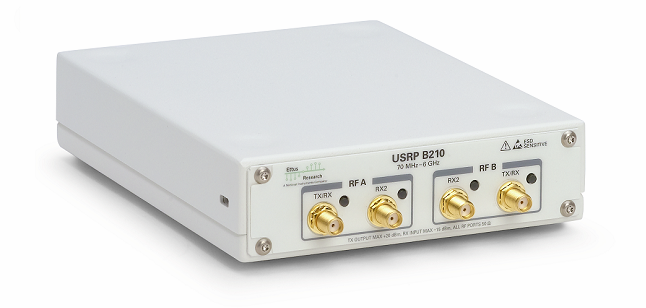
\includegraphics[width=0.7\linewidth]{figures/b210}
        \caption{USRP B210}
        \label{fig:b210}
    \end{subfigure}
    \begin{subfigure}[htb]{0.45\textwidth}
        \centering
        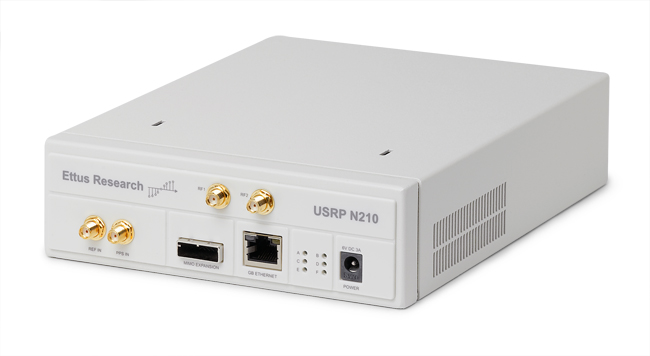
\includegraphics[width=0.7\linewidth]{figures/n210}
        \caption{USRP N210}
        \label{fig:n210}
    \end{subfigure}
    \begin{subfigure}[htb]{0.5\textwidth}
        \centering
        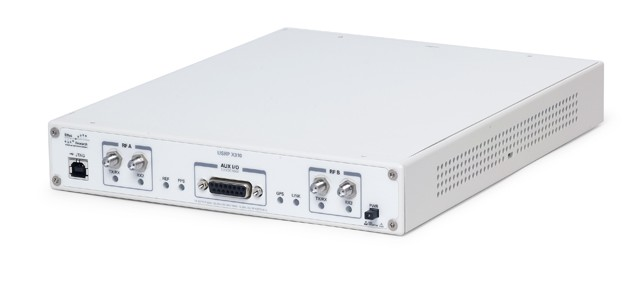
\includegraphics[width=0.7\linewidth]{figures/x310}
        \caption{USRP X300}
        \label{fig:x300}
    \end{subfigure}
    \begin{subfigure}[htb]{0.4\textwidth}
        \centering
        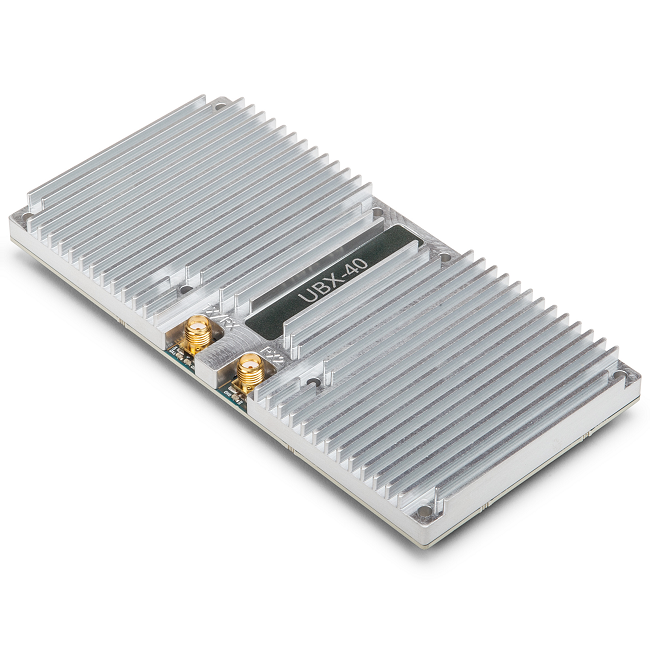
\includegraphics[width=0.6\linewidth]{figures/UBX40}
        \caption{UBX-40 daughterboard}
        \label{fig:UBX}
    \end{subfigure}
    \caption{\ac{USRP} Devices used in the complete DySpan challenge setup}
    \label{fig:ettus}
\end{figure}

For this thesis, the \ac{SU} implementation is reproduced, for which the N210 as transmitter and the B210 as receiver are used.

\section{Machine Learning models in Python and Jupyter}
\begin{figure}[!h]
    \centering
    \begin{subfigure}[htb]{0.45\textwidth}
        \centering
        
\includegraphics[width=\linewidth]{figures/python_logo}
        \label{fig:python}
    \end{subfigure}
    \begin{subfigure}[htb]{0.45\textwidth}
        \centering
        
\includegraphics[width=\linewidth]{figures/jupyter_logo}
        \label{fig:jupyter}
    \end{subfigure}
    \caption{Python and Jupyter logos}
    \label{fig:python_jupyter}
\end{figure}
For the learning part of this work, the focus on the implementation was given to a couple of popular Python libraries that have been effective when dealing with \ac{ML} problems: scikit-learn \cite{SKLEARN} and keras \cite{KERAS}. This libraries were chosen because of the simplicity of their prototyping as well as their effectiveness when providing an implementation that suits the \ac{ML} needs by returning fully trained models with exceptional prediction accuracy, and are described in more detail in the following sections. Additionally, the fact that these libraries are written in Python raises interest because this means that they interface optimally with GNURadio, making the inclussion of these libraries transparent, and having the perks of Python such as easy debugging and extensibility.\\

As for model testing and visualization, Jupyter notebooks \cite{Jupyter} have been used and are presented as part of the code repository of this thesis. What Jupyter provides is an open-source web application in which a number of interpreters for languages such as Python, R, Julia and Scala are embedded, allowing the creation and sharing of interactive register that contains code lines and excecution output along with visualization fields for plots and graphs and documentation in markdown, in what is called \emph{literate programming}. These notebooks can be shared in multiple formats, such as the native notebook format (for further modification of its contents), as well as HTML, \LaTeX{} and PDF (generated with \LaTeX). Moreover, it is nicely integrated with GitHub, so that the notebook can be visualized in the webpage of a remote repository without the need of conversion.\\

Jupyter is the continuation of a long effort for supporting interactive Python interpreters - the IPython Project \cite{IPython}. It has had a bast adoption in the last few years, such that even complete books have been written only using Jupyter as their interface for text editing and code examples. One of the main sources used for this work \cite{Andreas} is one example of such.

\subsection{Scikit-learn}
\begin{figure}[!h]
    \centering
    
\includegraphics[width=0.4\linewidth]{figures/sklearn_logo}
    \label{fig:sklearn_logo}
    \caption{Scikit-learn logo}
\end{figure}
Scikit-learn, formerly scikits.learn and also known as sklearn, is \ac{ML} library that features an abundance of algorithms for supervised and unsupervised algorithms, including the ones described in section~\ref{ch:ml_algs}. This library came as a result from a \emph{Google Summer of Code} project as a third party extension to SciPy, from where it gets its name. This library was used in this thesis for all the learning based on the extracted features listed in section~\ref{ch:features}.

\subsection{Keras}
\begin{figure}[!h]
    \centering
    
\includegraphics[width=0.5\linewidth]{figures/keras_logo}
    \label{fig:keras_logo}
    \caption{Keras logo}
\end{figure}
Keras is a high-level neural networks API written in Python that uses TensorFlow \cite{TensorFlow}, CNTK \cite{CNTK} or Theano \cite{Theano} as a backend. The way it is written in a way that allows datascientist to prototype and experiment fast. As per its documentation \cite{KERAS}:\emph{"being able to go from idea to result with the least possible delay is key to doing good research"}, and Keras certainly intends to keep the coding part as simple as possible for the designer to focus on the idea and not the programming of it. For this, it presents and API that is:

\begin{itemize}
    \item User-friendly: with ease for writing, reading and understanding.
    \item Modular: models have a clear begin and end, and they can be easily connected with other models with low to none restrictions.
    \item  Extendible: new functionalities and features are easily added to the mainstream, and the existing codebase is well-documented and exemplified.
\end{itemize}

For this project, Keras is used for convolutional neural networks implementation, using Tensorflow (with GPU support) as a backend.

\section{Data set Generation}
This part of the work regards the steps taken in order to have the data ready for the \ac{ML} algorithms to learn from it. It covers the testbed setup, the raw data (I/Q samples) measurement, and the data preprocessing.
\subsection{Measure Campaign}
The first step taken was to set up the \ac{PU} communication link over the air, and recording the raw samples just as the \ac{SU} would be able to "hear" them. The measurement setup is shown in Fig~\ref{fig:measurement}, where two parts are labeled separately.

\begin{figure}[!htb]
    \centering
    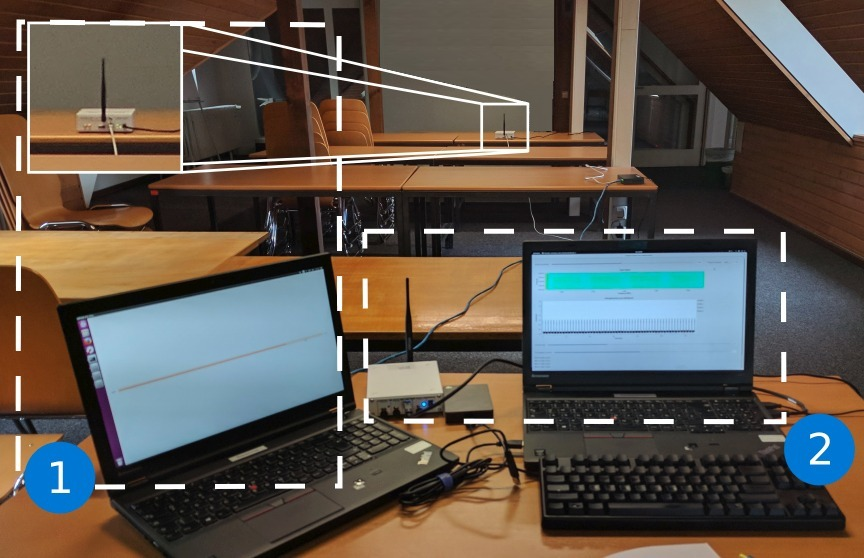
\includegraphics[width=0.5\linewidth]{figures/mod}
    \label{fig:measurement}
    \caption{Measurement Setup}
\end{figure}

The part labeled with \textcircled{1} regards the transmission part, which is going to be sending frames over the air in ten different fashions, described in Table~\ref{table:scenarios}.  The host machine in this part has the connection to the database, from where the information frames are extracted and put as payload of the transmitted frames. Additionally, the GNURadio flowgraph that generates the signal, which can be seen in Fig~\ref{fig:PU_flowgraph}, is also hosted and run from this computer. A summary of the path that a frame travels from the database until the transmitter is as follows: in Fig.~\ref{fig:PU_flowgraph} it can be seen that a connection to the database is done in the "Cmd pktgen" block, which is in charge of retreiving the information frames from the database, in form of \ac{PDU}, and feeding them into the signal processing blocks. After converting the \ac{PDU} into a tagged stream (a stream of data that has metadata attached to it in form of tags), the stream flows into the \ac{OFDM} transmitter block, which is a hierarchical block that allocates the carriers for an \ac{OFDM} transmission, applies a \ac{FFT} to them, and appends a cyclic prefix.

\begin{figure}[!htb]
    \centering
    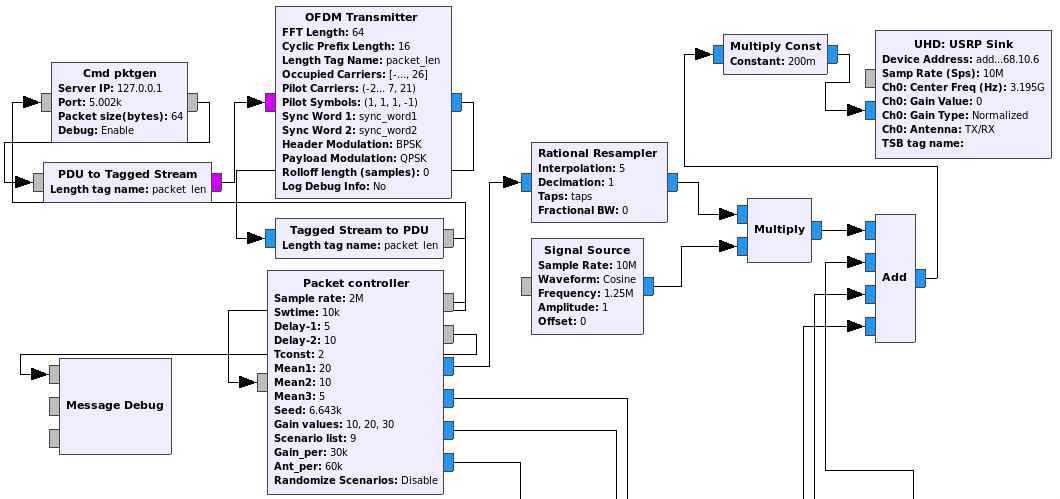
\includegraphics[width=\textwidth]{figures/PU_flowgraph}
    \label{fig:PU_flowgraph}
    \caption{\ac{PU} GNURadio flowgraph}
\end{figure}

\subsection{Feature Engineering}\label{ch:features}
\subsection{Spectrograms generation}
